\documentclass[../../thesis.tex]{subfiles}

\begin{document}
Our work in this thesis can be seen as a tangent of the paper "Vector Quantized Time Series Generation with a Bidirectional Prior Model" \cite{TimeVQVAE}. 
We simplify the model architecture by omitting the high-low frequency split, which reduces the model to what they refer to as naive TimeVQVAE in their paper. We expand on naive TimeVQVAE  with a self-supervised extension. \newline

A schematic figure of our proposed tokenization model is given in \ref{fig:NCVQVAE}. To improve on the reconstruction we add a regularizing term by reconstructing augmented views. We hypothesize that the model generalizes better to unseen data by letting the decoder "see" the augmented views.\newline
To separate classes better we introduce a non contrastive self supervised loss. The intuition being that the representation of original and augmented views are pushed closer together by the SSL loss.\newline

\section{Proposed model: NC-VQVAE}

Our model, termed NC-VQVAE, is a generative time series model which learns expressive discrete latent representations by combining VQVAE \cite{VQVAE} with non contrastive self supervised learning algorithms. NC-VQVAE uses the two staged modelling approach presented in \cite{TimeVQVAE}, and can be considered an extension of their "naive TimeVQVAE". Our model mainly extends the tokenization stage, where we incorporate Barlow Twins \cite{zbontar2021barlow} and VIbCReg \cite{lee2024computer} as our non contrastive SSL, but the framework is flexible. For stage two we model the prior using a bidirectional transformer as MaskGIT \cite{chang2022maskgit}.

\subsection{Stage 1: Tokenization}

The architecture of the tokenization model \ref{fig:NCVQVAE} consists of two branches. The top and bottom branch is referred to as the original and augmented branch respectively. The model takes a time series $x$ as input and creates an augmented view $x'$. The original branch is simply the naive TimeVQVAE from \cite{TimeVQVAE}, while the augmented branch is an autoencoder, constructed by omitting the quantization layer. The views are passed through their respective branches, where we compute the SSL loss derived from the original discrete latent representation $z_q$ and the augmented continuous latent $z'$, before the decoder reconstructs each latent representation. \newline 
The SSL loss is calculated by concatenate the global average and max pool of both representations individually and passing the resulting vectors through the projector. \newline

\begin{figure}[h]
    \label{fig:NCVQVAE}
    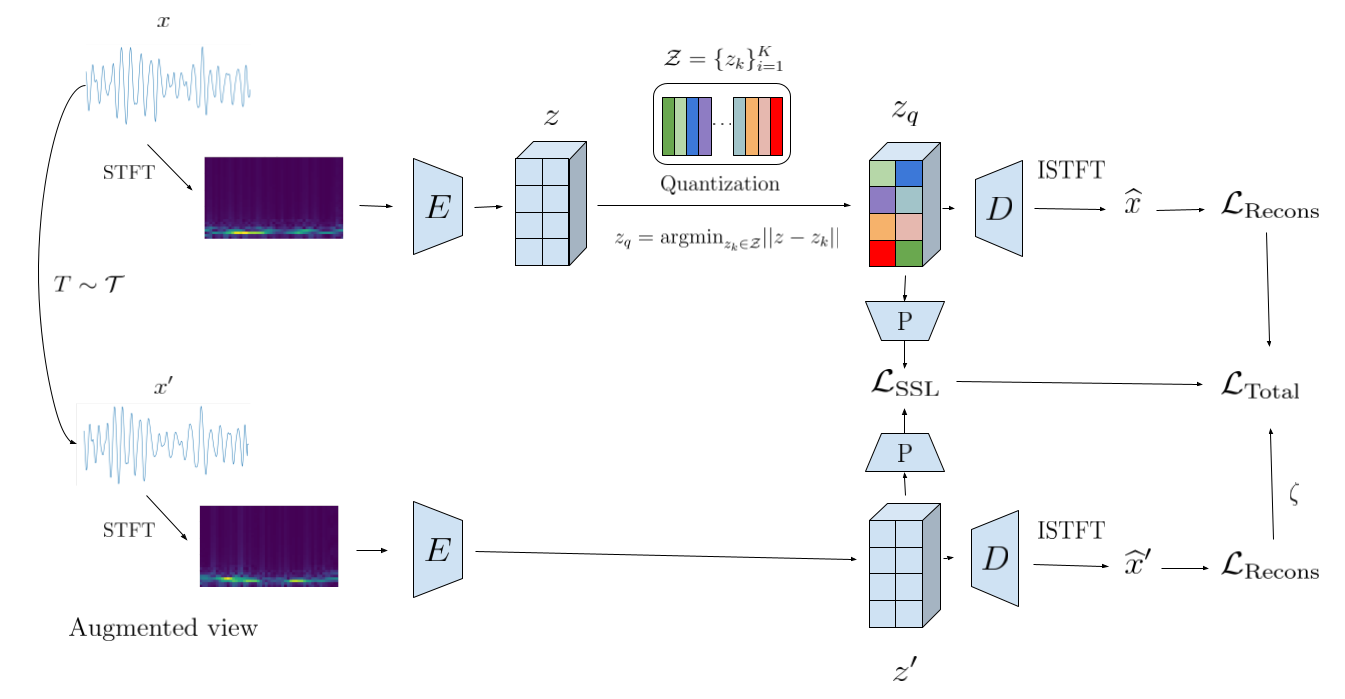
\includegraphics[scale=0.27]{Siam-VQVAE.png}
    \centering  
    \caption{Overview of proposed model. NC-VQVAE. Fix index on Z, add weight to arrow from ssl loss to total. fix argmin index thing.}
\end{figure}

\subsubsection{Loss}
Our training objective reflects the training objective from TimeVQVAE in equation \ref{eq:TimeVQVAE_loss} without the frequency split. Our contribution is the addition of a SLL loss together with a reconstruction loss on the augmented branch.\newline

To refresh the readers memory the VQ loss consists of a reconstruction loss, codebook loss which is the MSE of continuous and discrete latent representations together with a commitment loss which keeps the codewords from diverging. In our setup the codebook loss reduces to
\begin{equation}
    \label{eq:NCVQVAE_codebook}
    \begin{aligned}
        \loss_\text{codebook} &= ||\sg[z] - z_q ||_2^2 \\
                              &+ \beta||z - \sg[z_q]||_2^2,
    \end{aligned}
\end{equation}

and the reconstruction loss to
\begin{equation}
    \label{eq:NCVQVAE_recons}
        \loss_\text{recons} = ||x - \widehat{x} ||_2^2 + ||u - \widehat{u}||_2^2.
\end{equation}
\newline
Our VQ loss is too given by
\begin{equation}
    \label{eq:NCVQVAE_loss}
    \loss_\text{VQ} = \loss_\text{codebook} + \loss_\text{recons}.
\end{equation}

The SSL loss takes form depending on which SSL method used. The loss is calculated on derived values from $z_q$ and $z'$. In our work we consider Barlow Twins \ref{eq:BTLoss} and VIbCReg \ref{eq:VIbCRegLoss}, both of which utilizes a projector. We apply a global average and max pool operation on both tensors and pass them through the projector before calculating the 
The discrete latent representations from the original branch and the continuous latent representations from the augmented branch are pushed to similar regions of latent space.
\newline

The augmented reconstruction loss is simply given as 
\begin{equation}
    \label{eq:NCVQVAE_augrecons}
        \loss_\text{recons}' = ||x' - \widehat{x}' ||_2^2 + ||u' - \widehat{u}'||_2^2,
\end{equation}

and provides the encoder and decoder with instructions to reconstruct the augmented view, which in conjunction with the SSL loss, influence the codebook to encode information regarding the augmentations. Additionally we hypothesize that it assists the encoder in not ignoring reconstruction on behalf of the SSL loss. During initial testing, omitting the augmentation reconstruction lead to severe overfitting.\newline

The total loss is given by 
\begin{equation}
    \loss_{NC-VQVAE} = \loss_{VQ} + \eta\loss_{\text{SSL}} + \zeta \loss_\text{recons}',
\end{equation}
where $\eta$ and $\zeta$ are hyperparameters influencing the importance of the terms for the total training objective. 


\subsection{Stage 2: Prior learning}

In our model the input embedding for the bidirectional transformer is initialized with the codebook with learned structure from both reconstruction and SSL loss. Instead of introducing an additional masking vector in the embedding matrix, we rather use the codebook directly, and create a separate learnable masking vector, and mask the embedded sequences using this. The only difference between our proposal and the mechanism used in MaskGIT and TimeVQVAE is that the learning of the masked token embedding is independent of the other embeddings, i.e it is not influenced and does not influence by the learning of the finetuned codebook. The rationality behind this is to further leverage and not unnecessarily influence the learned codewords from stage 1. Except for this adjustment and the possibility of class conditional sampling from TimeVQVAE, our method is equivalent to MaskGITs.
\newline

In order to separate this masking vector, we do the embedding stage before masking, effectively factoring the embedding out of the transformer. The generation procedure is identical to the iterative decoding from MaskGIT. 



\end{document}